\documentclass[1p]{elsarticle_modified}
%\bibliographystyle{elsarticle-num}

%\usepackage[colorlinks]{hyperref}
%\usepackage{abbrmath_seonhwa} %\Abb, \Ascr, \Acal ,\Abf, \Afrak
\usepackage{amsfonts}
\usepackage{amssymb}
\usepackage{amsmath}
\usepackage{amsthm}
\usepackage{scalefnt}
\usepackage{amsbsy}
\usepackage{kotex}
\usepackage{caption}
\usepackage{subfig}
\usepackage{color}
\usepackage{graphicx}
\usepackage{xcolor} %% white, black, red, green, blue, cyan, magenta, yellow
\usepackage{float}
\usepackage{setspace}
\usepackage{hyperref}

\usepackage{tikz}
\usetikzlibrary{arrows}

\usepackage{multirow}
\usepackage{array} % fixed length table
\usepackage{hhline}

%%%%%%%%%%%%%%%%%%%%%
\makeatletter
\renewcommand*\env@matrix[1][\arraystretch]{%
	\edef\arraystretch{#1}%
	\hskip -\arraycolsep
	\let\@ifnextchar\new@ifnextchar
	\array{*\c@MaxMatrixCols c}}
\makeatother %https://tex.stackexchange.com/questions/14071/how-can-i-increase-the-line-spacing-in-a-matrix
%%%%%%%%%%%%%%%

\usepackage[normalem]{ulem}

\newcommand{\msout}[1]{\ifmmode\text{\sout{\ensuremath{#1}}}\else\sout{#1}\fi}
%SOURCE: \msout is \stkout macro in https://tex.stackexchange.com/questions/20609/strikeout-in-math-mode

\newcommand{\cancel}[1]{
	\ifmmode
	{\color{red}\msout{#1}}
	\else
	{\color{red}\sout{#1}}
	\fi
}

\newcommand{\add}[1]{
	{\color{blue}\uwave{#1}}
}

\newcommand{\replace}[2]{
	\ifmmode
	{\color{red}\msout{#1}}{\color{blue}\uwave{#2}}
	\else
	{\color{red}\sout{#1}}{\color{blue}\uwave{#2}}
	\fi
}

\newcommand{\Sol}{\mathcal{S}} %segment
\newcommand{\D}{D} %diagram
\newcommand{\A}{\mathcal{A}} %arc


%%%%%%%%%%%%%%%%%%%%%%%%%%%%%5 test

\def\sl{\operatorname{\textup{SL}}(2,\Cbb)}
\def\psl{\operatorname{\textup{PSL}}(2,\Cbb)}
\def\quan{\mkern 1mu \triangleright \mkern 1mu}

\theoremstyle{definition}
\newtheorem{thm}{Theorem}[section]
\newtheorem{prop}[thm]{Proposition}
\newtheorem{lem}[thm]{Lemma}
\newtheorem{ques}[thm]{Question}
\newtheorem{cor}[thm]{Corollary}
\newtheorem{defn}[thm]{Definition}
\newtheorem{exam}[thm]{Example}
\newtheorem{rmk}[thm]{Remark}
\newtheorem{alg}[thm]{Algorithm}

\newcommand{\I}{\sqrt{-1}}
\begin{document}

%\begin{frontmatter}
%
%\title{Boundary parabolic representations of knots up to 8 crossings}
%
%%% Group authors per affiliation:
%\author{Yunhi Cho} 
%\address{Department of Mathematics, University of Seoul, Seoul, Korea}
%\ead{yhcho@uos.ac.kr}
%
%
%\author{Seonhwa Kim} %\fnref{s_kim}}
%\address{Center for Geometry and Physics, Institute for Basic Science, Pohang, 37673, Korea}
%\ead{ryeona17@ibs.re.kr}
%
%\author{Hyuk Kim}
%\address{Department of Mathematical Sciences, Seoul National University, Seoul 08826, Korea}
%\ead{hyukkim@snu.ac.kr}
%
%\author{Seokbeom Yoon}
%\address{Department of Mathematical Sciences, Seoul National University, Seoul, 08826,  Korea}
%\ead{sbyoon15@snu.ac.kr}
%
%\begin{abstract}
%We find all boundary parabolic representation of knots up to 8 crossings.
%
%\end{abstract}
%\begin{keyword}
%    \MSC[2010] 57M25 
%\end{keyword}
%
%\end{frontmatter}

%\linenumbers
%\tableofcontents
%
\newcommand\colored[1]{\textcolor{white}{\rule[-0.35ex]{0.8em}{1.4ex}}\kern-0.8em\color{red} #1}%
%\newcommand\colored[1]{\textcolor{white}{ #1}\kern-2.17ex	\textcolor{white}{ #1}\kern-1.81ex	\textcolor{white}{ #1}\kern-2.15ex\color{red}#1	}

{\Large $\underline{12n_{0358}~(K12n_{0358})}$}

\setlength{\tabcolsep}{10pt}
\renewcommand{\arraystretch}{1.6}
\vspace{1cm}\begin{tabular}{m{100pt}>{\centering\arraybackslash}m{274pt}}
\multirow{5}{120pt}{
	\centering
	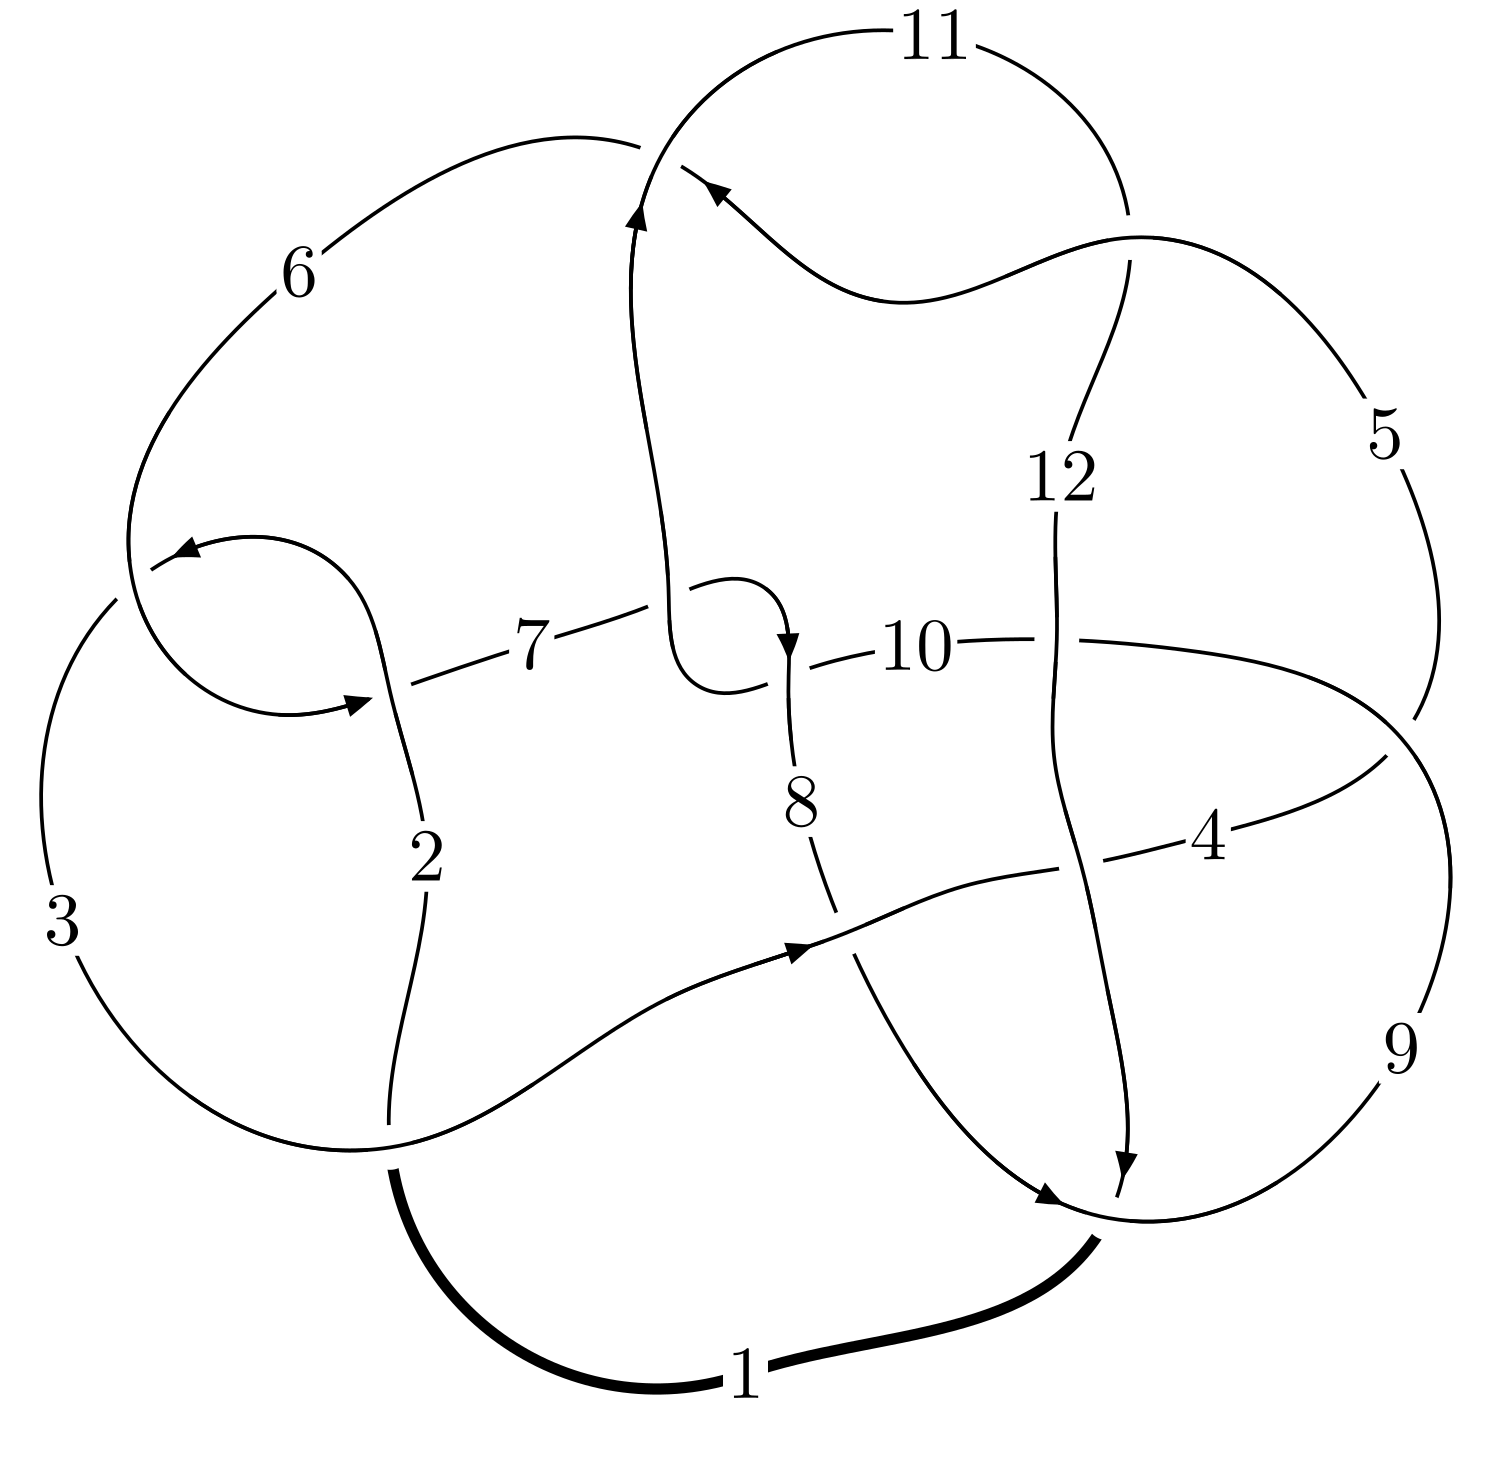
\includegraphics[width=112pt]{../../../GIT/diagram.site/Diagrams/png/2447_12n_0358.png}\\
\ \ \ A knot diagram\footnotemark}&
\allowdisplaybreaks
\textbf{Linearized knot diagam} \\
\cline{2-2}
 &
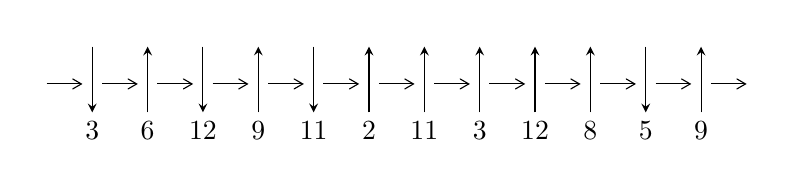
\begin{tikzpicture}[x=20pt, y=17pt]
	% nodes
	\node (C0) at (0, 0) {};
	\node (C1) at (1, 0) {};
	\node (C1U) at (1, +1) {};
	\node (C1D) at (1, -1) {3};

	\node (C2) at (2, 0) {};
	\node (C2U) at (2, +1) {};
	\node (C2D) at (2, -1) {6};

	\node (C3) at (3, 0) {};
	\node (C3U) at (3, +1) {};
	\node (C3D) at (3, -1) {12};

	\node (C4) at (4, 0) {};
	\node (C4U) at (4, +1) {};
	\node (C4D) at (4, -1) {9};

	\node (C5) at (5, 0) {};
	\node (C5U) at (5, +1) {};
	\node (C5D) at (5, -1) {11};

	\node (C6) at (6, 0) {};
	\node (C6U) at (6, +1) {};
	\node (C6D) at (6, -1) {2};

	\node (C7) at (7, 0) {};
	\node (C7U) at (7, +1) {};
	\node (C7D) at (7, -1) {11};

	\node (C8) at (8, 0) {};
	\node (C8U) at (8, +1) {};
	\node (C8D) at (8, -1) {3};

	\node (C9) at (9, 0) {};
	\node (C9U) at (9, +1) {};
	\node (C9D) at (9, -1) {12};

	\node (C10) at (10, 0) {};
	\node (C10U) at (10, +1) {};
	\node (C10D) at (10, -1) {8};

	\node (C11) at (11, 0) {};
	\node (C11U) at (11, +1) {};
	\node (C11D) at (11, -1) {5};

	\node (C12) at (12, 0) {};
	\node (C12U) at (12, +1) {};
	\node (C12D) at (12, -1) {9};
	\node (C13) at (13, 0) {};

	% arrows
	\draw[->,>={angle 60}]
	(C0) edge (C1) (C1) edge (C2) (C2) edge (C3) (C3) edge (C4) (C4) edge (C5) (C5) edge (C6) (C6) edge (C7) (C7) edge (C8) (C8) edge (C9) (C9) edge (C10) (C10) edge (C11) (C11) edge (C12) (C12) edge (C13) ;	\draw[->,>=stealth]
	(C1U) edge (C1D) (C2D) edge (C2U) (C3U) edge (C3D) (C4D) edge (C4U) (C5U) edge (C5D) (C6D) edge (C6U) (C7D) edge (C7U) (C8D) edge (C8U) (C9D) edge (C9U) (C10D) edge (C10U) (C11U) edge (C11D) (C12D) edge (C12U) ;
	\end{tikzpicture} \\
\hhline{~~} \\& 
\textbf{Solving Sequence} \\ \cline{2-2} 
 &
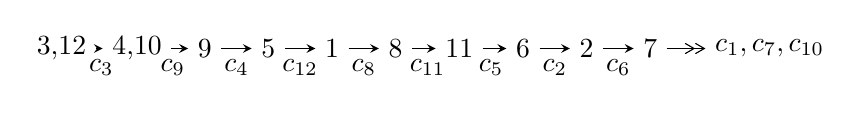
\begin{tikzpicture}[x=23pt, y=7pt]
	% node
	\node (A0) at (-1/8, 0) {3,12};
	\node (A1) at (17/16, 0) {4,10};
	\node (A2) at (17/8, 0) {9};
	\node (A3) at (25/8, 0) {5};
	\node (A4) at (33/8, 0) {1};
	\node (A5) at (41/8, 0) {8};
	\node (A6) at (49/8, 0) {11};
	\node (A7) at (57/8, 0) {6};
	\node (A8) at (65/8, 0) {2};
	\node (A9) at (73/8, 0) {7};
	\node (C1) at (1/2, -1) {$c_{3}$};
	\node (C2) at (13/8, -1) {$c_{9}$};
	\node (C3) at (21/8, -1) {$c_{4}$};
	\node (C4) at (29/8, -1) {$c_{12}$};
	\node (C5) at (37/8, -1) {$c_{8}$};
	\node (C6) at (45/8, -1) {$c_{11}$};
	\node (C7) at (53/8, -1) {$c_{5}$};
	\node (C8) at (61/8, -1) {$c_{2}$};
	\node (C9) at (69/8, -1) {$c_{6}$};
	\node (A10) at (11, 0) {$c_{1},c_{7},c_{10}$};

	% edge
	\draw[->,>=stealth]	
	(A0) edge (A1) (A1) edge (A2) (A2) edge (A3) (A3) edge (A4) (A4) edge (A5) (A5) edge (A6) (A6) edge (A7) (A7) edge (A8) (A8) edge (A9) ;
	\draw[->>,>={angle 60}]	
	(A9) edge (A10);
\end{tikzpicture} \\ 

\end{tabular} \\

\footnotetext{
The image of knot diagram is generated by the software ``\textbf{Draw programme}" developed by Andrew Bartholomew(\url{http://www.layer8.co.uk/maths/draw/index.htm\#Running-draw}), where we modified some parts for our purpose(\url{https://github.com/CATsTAILs/LinksPainter}).
}\phantom \\ \newline 
\centering \textbf{Ideals for irreducible components\footnotemark of $X_{\text{par}}$} 
 
\begin{align*}
I^u_{1}&=\langle 
-1.46895\times10^{55} u^{31}-2.31201\times10^{55} u^{30}+\cdots+5.76616\times10^{56} b+7.64769\times10^{56},\\
\phantom{I^u_{1}}&\phantom{= \langle  }-2.64393\times10^{56} u^{31}-4.61405\times10^{56} u^{30}+\cdots+4.90124\times10^{57} a-2.09273\times10^{58},\\
\phantom{I^u_{1}}&\phantom{= \langle  }u^{32}+u^{31}+\cdots-115 u+17\rangle \\
I^u_{2}&=\langle 
213 u^{10}+543 u^9+\cdots+122 b+729,\\
\phantom{I^u_{2}}&\phantom{= \langle  }-7 u^{10}-84 u^9-87 u^8+359 u^7+671 u^6+340 u^5-74 u^4-1583 u^3-2753 u^2+61 a-2059 u-713,\\
\phantom{I^u_{2}}&\phantom{= \langle  }u^{11}+2 u^{10}-3 u^9-10 u^8-10 u^7-5 u^6+17 u^5+42 u^4+49 u^3+30 u^2+10 u+1\rangle \\
\\
\end{align*}
\raggedright * 2 irreducible components of $\dim_{\mathbb{C}}=0$, with total 43 representations.\\
\footnotetext{All coefficients of polynomials are rational numbers. But the coefficients are sometimes approximated in decimal forms when there is not enough margin.}
\newpage
\renewcommand{\arraystretch}{1}
\centering \section*{I. $I^u_{1}= \langle -1.47\times10^{55} u^{31}-2.31\times10^{55} u^{30}+\cdots+5.77\times10^{56} b+7.65\times10^{56},\;-2.64\times10^{56} u^{31}-4.61\times10^{56} u^{30}+\cdots+4.90\times10^{57} a-2.09\times10^{58},\;u^{32}+u^{31}+\cdots-115 u+17 \rangle$}
\flushleft \textbf{(i) Arc colorings}\\
\begin{tabular}{m{7pt} m{180pt} m{7pt} m{180pt} }
\flushright $a_{3}=$&$\begin{pmatrix}1\\0\end{pmatrix}$ \\
\flushright $a_{12}=$&$\begin{pmatrix}0\\u\end{pmatrix}$ \\
\flushright $a_{4}=$&$\begin{pmatrix}1\\u^2\end{pmatrix}$ \\
\flushright $a_{10}=$&$\begin{pmatrix}0.0539440 u^{31}+0.0941405 u^{30}+\cdots-13.7837 u+4.26980\\0.0254754 u^{31}+0.0400962 u^{30}+\cdots+7.97722 u-1.32630\end{pmatrix}$ \\
\flushright $a_{9}=$&$\begin{pmatrix}0.0539440 u^{31}+0.0941405 u^{30}+\cdots-13.7837 u+4.26980\\0.0325030 u^{31}+0.0420930 u^{30}+\cdots+11.6828 u-2.00964\end{pmatrix}$ \\
\flushright $a_{5}=$&$\begin{pmatrix}-0.153248 u^{31}-0.190779 u^{30}+\cdots-49.4372 u+5.45094\\-0.00183023 u^{31}-0.00426829 u^{30}+\cdots+1.54109 u+0.765218\end{pmatrix}$ \\
\flushright $a_{1}=$&$\begin{pmatrix}-0.127739 u^{31}-0.125659 u^{30}+\cdots-66.7508 u+19.1973\\0.0366181 u^{31}+0.0475649 u^{30}+\cdots+16.5833 u-2.64057\end{pmatrix}$ \\
\flushright $a_{8}=$&$\begin{pmatrix}0.0214410 u^{31}+0.0520475 u^{30}+\cdots-25.4665 u+6.27945\\0.0325030 u^{31}+0.0420930 u^{30}+\cdots+11.6828 u-2.00964\end{pmatrix}$ \\
\flushright $a_{11}=$&$\begin{pmatrix}-0.0632575 u^{31}-0.110415 u^{30}+\cdots+10.2857 u-6.75211\\-0.00420108 u^{31}+0.0133699 u^{30}+\cdots-8.89145 u+2.02845\end{pmatrix}$ \\
\flushright $a_{6}=$&$\begin{pmatrix}0.0507264 u^{31}+0.0363812 u^{30}+\cdots+48.1205 u-4.78017\\-0.0492231 u^{31}-0.0588019 u^{30}+\cdots-14.1421 u+1.87216\end{pmatrix}$ \\
\flushright $a_{2}=$&$\begin{pmatrix}-0.164357 u^{31}-0.173224 u^{30}+\cdots-83.3341 u+21.8378\\0.0366181 u^{31}+0.0475649 u^{30}+\cdots+16.5833 u-2.64057\end{pmatrix}$ \\
\flushright $a_{7}=$&$\begin{pmatrix}-0.236694 u^{31}-0.382377 u^{30}+\cdots+10.7177 u-15.9857\\-0.0368276 u^{31}-0.0192369 u^{30}+\cdots-25.8376 u+5.99491\end{pmatrix}$\\&\end{tabular}
\flushleft \textbf{(ii) Obstruction class $= -1$}\\~\\
\flushleft \textbf{(iii) Cusp Shapes $= 0.163697 u^{31}+0.228954 u^{30}+\cdots+26.1806 u-4.32625$}\\~\\
\newpage\renewcommand{\arraystretch}{1}
\flushleft \textbf{(iv) u-Polynomials at the component}\newline \\
\begin{tabular}{m{50pt}|m{274pt}}
Crossings & \hspace{64pt}u-Polynomials at each crossing \\
\hline $$\begin{aligned}c_{1}\end{aligned}$$&$\begin{aligned}
&u^{32}+6 u^{31}+\cdots-18 u+1
\end{aligned}$\\
\hline $$\begin{aligned}c_{2},c_{6}\end{aligned}$$&$\begin{aligned}
&u^{32}-2 u^{31}+\cdots-6 u-1
\end{aligned}$\\
\hline $$\begin{aligned}c_{3}\end{aligned}$$&$\begin{aligned}
&u^{32}+u^{31}+\cdots-115 u+17
\end{aligned}$\\
\hline $$\begin{aligned}c_{4}\end{aligned}$$&$\begin{aligned}
&u^{32}+13 u^{30}+\cdots-632 u+247
\end{aligned}$\\
\hline $$\begin{aligned}c_{5},c_{11}\end{aligned}$$&$\begin{aligned}
&u^{32}+17 u^{30}+\cdots-8 u+4
\end{aligned}$\\
\hline $$\begin{aligned}c_{7},c_{10}\end{aligned}$$&$\begin{aligned}
&u^{32}+5 u^{31}+\cdots+441 u+43
\end{aligned}$\\
\hline $$\begin{aligned}c_{8}\end{aligned}$$&$\begin{aligned}
&u^{32}- u^{31}+\cdots-84 u-4
\end{aligned}$\\
\hline $$\begin{aligned}c_{9},c_{12}\end{aligned}$$&$\begin{aligned}
&u^{32}+18 u^{30}+\cdots-66 u+4
\end{aligned}$\\
\hline
\end{tabular}\\~\\
\newpage\renewcommand{\arraystretch}{1}
\flushleft \textbf{(v) Riley Polynomials at the component}\newline \\
\begin{tabular}{m{50pt}|m{274pt}}
Crossings & \hspace{64pt}Riley Polynomials at each crossing \\
\hline $$\begin{aligned}c_{1}\end{aligned}$$&$\begin{aligned}
&y^{32}+46 y^{31}+\cdots-70 y+1
\end{aligned}$\\
\hline $$\begin{aligned}c_{2},c_{6}\end{aligned}$$&$\begin{aligned}
&y^{32}+6 y^{31}+\cdots-18 y+1
\end{aligned}$\\
\hline $$\begin{aligned}c_{3}\end{aligned}$$&$\begin{aligned}
&y^{32}-39 y^{31}+\cdots+1565 y+289
\end{aligned}$\\
\hline $$\begin{aligned}c_{4}\end{aligned}$$&$\begin{aligned}
&y^{32}+26 y^{31}+\cdots+560418 y+61009
\end{aligned}$\\
\hline $$\begin{aligned}c_{5},c_{11}\end{aligned}$$&$\begin{aligned}
&y^{32}+34 y^{31}+\cdots+2096 y+16
\end{aligned}$\\
\hline $$\begin{aligned}c_{7},c_{10}\end{aligned}$$&$\begin{aligned}
&y^{32}-17 y^{31}+\cdots-40025 y+1849
\end{aligned}$\\
\hline $$\begin{aligned}c_{8}\end{aligned}$$&$\begin{aligned}
&y^{32}+17 y^{31}+\cdots-6688 y+16
\end{aligned}$\\
\hline $$\begin{aligned}c_{9},c_{12}\end{aligned}$$&$\begin{aligned}
&y^{32}+36 y^{31}+\cdots-524 y+16
\end{aligned}$\\
\hline
\end{tabular}\\~\\
\newpage\flushleft \textbf{(vi) Complex Volumes and Cusp Shapes}
$$\begin{array}{c|c|c}  
\text{Solutions to }I^u_{1}& \I (\text{vol} + \sqrt{-1}CS) & \text{Cusp shape}\\
 \hline 
\begin{aligned}
u &= \phantom{-}0.890291 + 0.082335 I \\
a &= -0.189708 - 1.127940 I \\
b &= -1.42359 + 0.30650 I\end{aligned}
 & \phantom{-}5.53757 + 4.69649 I & \phantom{-}5.81138 - 4.02959 I \\ \hline\begin{aligned}
u &= \phantom{-}0.890291 - 0.082335 I \\
a &= -0.189708 + 1.127940 I \\
b &= -1.42359 - 0.30650 I\end{aligned}
 & \phantom{-}5.53757 - 4.69649 I & \phantom{-}5.81138 + 4.02959 I \\ \hline\begin{aligned}
u &= \phantom{-}1.161750 + 0.190152 I \\
a &= -0.786860 - 1.073630 I \\
b &= \phantom{-}0.379154 + 1.290560 I\end{aligned}
 & -0.43634 + 3.10421 I & \phantom{-}4.37459 - 4.74046 I \\ \hline\begin{aligned}
u &= \phantom{-}1.161750 - 0.190152 I \\
a &= -0.786860 + 1.073630 I \\
b &= \phantom{-}0.379154 - 1.290560 I\end{aligned}
 & -0.43634 - 3.10421 I & \phantom{-}4.37459 + 4.74046 I \\ \hline\begin{aligned}
u &= -1.175740 + 0.411357 I \\
a &= -0.127425 + 1.003260 I \\
b &= \phantom{-}1.033100 - 0.703261 I\end{aligned}
 & \phantom{-}4.08919 - 2.13529 I & \phantom{-}6.31237 + 2.22583 I \\ \hline\begin{aligned}
u &= -1.175740 - 0.411357 I \\
a &= -0.127425 - 1.003260 I \\
b &= \phantom{-}1.033100 + 0.703261 I\end{aligned}
 & \phantom{-}4.08919 + 2.13529 I & \phantom{-}6.31237 - 2.22583 I \\ \hline\begin{aligned}
u &= \phantom{-}0.363496 + 0.633573 I \\
a &= -0.863446 + 0.181273 I \\
b &= \phantom{-}0.821719 + 0.702091 I\end{aligned}
 & \phantom{-}1.95190 + 1.49124 I & \phantom{-}11.14082 + 0.24484 I \\ \hline\begin{aligned}
u &= \phantom{-}0.363496 - 0.633573 I \\
a &= -0.863446 - 0.181273 I \\
b &= \phantom{-}0.821719 - 0.702091 I\end{aligned}
 & \phantom{-}1.95190 - 1.49124 I & \phantom{-}11.14082 - 0.24484 I \\ \hline\begin{aligned}
u &= -0.191542 + 0.580828 I \\
a &= -0.481932 + 0.510086 I \\
b &= -0.137918 + 0.496964 I\end{aligned}
 & \phantom{-}0.227121 + 1.283920 I & \phantom{-}2.61051 - 5.66757 I \\ \hline\begin{aligned}
u &= -0.191542 - 0.580828 I \\
a &= -0.481932 - 0.510086 I \\
b &= -0.137918 - 0.496964 I\end{aligned}
 & \phantom{-}0.227121 - 1.283920 I & \phantom{-}2.61051 + 5.66757 I\\
 \hline 
 \end{array}$$\newpage$$\begin{array}{c|c|c}  
\text{Solutions to }I^u_{1}& \I (\text{vol} + \sqrt{-1}CS) & \text{Cusp shape}\\
 \hline 
\begin{aligned}
u &= -0.586343 + 0.124328 I \\
a &= -0.609159 + 0.724747 I \\
b &= -0.877370 - 0.691695 I\end{aligned}
 & -1.63912 + 2.52987 I & -3.57474 - 4.78541 I \\ \hline\begin{aligned}
u &= -0.586343 - 0.124328 I \\
a &= -0.609159 - 0.724747 I \\
b &= -0.877370 + 0.691695 I\end{aligned}
 & -1.63912 - 2.52987 I & -3.57474 + 4.78541 I \\ \hline\begin{aligned}
u &= \phantom{-}0.580660\phantom{ +0.000000I} \\
a &= -0.308351\phantom{ +0.000000I} \\
b &= \phantom{-}1.06280\phantom{ +0.000000I}\end{aligned}
 & \phantom{-}1.60623\phantom{ +0.000000I} & \phantom{-}5.12950\phantom{ +0.000000I} \\ \hline\begin{aligned}
u &= -1.36973 + 0.80419 I \\
a &= \phantom{-}0.571260 - 0.450326 I \\
b &= \phantom{-}0.279827 + 1.286450 I\end{aligned}
 & -2.62185 + 1.74811 I & \phantom{-0.000000 } 0. - 2.22664 I \\ \hline\begin{aligned}
u &= -1.36973 - 0.80419 I \\
a &= \phantom{-}0.571260 + 0.450326 I \\
b &= \phantom{-}0.279827 - 1.286450 I\end{aligned}
 & -2.62185 - 1.74811 I & \phantom{-0.000000 -}0. + 2.22664 I \\ \hline\begin{aligned}
u &= \phantom{-}0.371814\phantom{ +0.000000I} \\
a &= -3.54305\phantom{ +0.000000I} \\
b &= \phantom{-}0.442169\phantom{ +0.000000I}\end{aligned}
 & \phantom{-}2.54557\phantom{ +0.000000I} & -5.58620\phantom{ +0.000000I} \\ \hline\begin{aligned}
u &= \phantom{-}1.60097 + 0.38950 I \\
a &= \phantom{-}0.162146 + 1.065720 I \\
b &= \phantom{-}0.32297 - 1.79367 I\end{aligned}
 & -5.37656 - 5.61867 I & \phantom{-0.000000 -}0. + 7.53419 I \\ \hline\begin{aligned}
u &= \phantom{-}1.60097 - 0.38950 I \\
a &= \phantom{-}0.162146 - 1.065720 I \\
b &= \phantom{-}0.32297 + 1.79367 I\end{aligned}
 & -5.37656 + 5.61867 I & \phantom{-0.000000 } 0. - 7.53419 I \\ \hline\begin{aligned}
u &= \phantom{-}0.103968 + 0.203519 I \\
a &= \phantom{-}4.04227 - 6.75624 I \\
b &= -0.033520 + 0.954984 I\end{aligned}
 & \phantom{-}8.08284 + 4.26134 I & \phantom{-}3.05142 - 2.81645 I \\ \hline\begin{aligned}
u &= \phantom{-}0.103968 - 0.203519 I \\
a &= \phantom{-}4.04227 + 6.75624 I \\
b &= -0.033520 - 0.954984 I\end{aligned}
 & \phantom{-}8.08284 - 4.26134 I & \phantom{-}3.05142 + 2.81645 I\\
 \hline 
 \end{array}$$\newpage$$\begin{array}{c|c|c}  
\text{Solutions to }I^u_{1}& \I (\text{vol} + \sqrt{-1}CS) & \text{Cusp shape}\\
 \hline 
\begin{aligned}
u &= -1.73055 + 0.44345 I \\
a &= -0.205729 + 0.838219 I \\
b &= -0.555914 - 1.276110 I\end{aligned}
 & -4.57570 + 2.93695 I & \phantom{-0.000000 } 0 \\ \hline\begin{aligned}
u &= -1.73055 - 0.44345 I \\
a &= -0.205729 - 0.838219 I \\
b &= -0.555914 + 1.276110 I\end{aligned}
 & -4.57570 - 2.93695 I & \phantom{-0.000000 } 0 \\ \hline\begin{aligned}
u &= -1.76860 + 0.43431 I \\
a &= -0.063506 - 1.029620 I \\
b &= \phantom{-}0.69370 + 1.26085 I\end{aligned}
 & \phantom{-}2.10446 + 4.39637 I & \phantom{-0.000000 } 0 \\ \hline\begin{aligned}
u &= -1.76860 - 0.43431 I \\
a &= -0.063506 + 1.029620 I \\
b &= \phantom{-}0.69370 - 1.26085 I\end{aligned}
 & \phantom{-}2.10446 - 4.39637 I & \phantom{-0.000000 } 0 \\ \hline\begin{aligned}
u &= \phantom{-}1.84685 + 0.19418 I \\
a &= \phantom{-}0.215144 + 0.971986 I \\
b &= -0.158364 - 1.139650 I\end{aligned}
 & -9.68142 + 0.70132 I & \phantom{-0.000000 } 0 \\ \hline\begin{aligned}
u &= \phantom{-}1.84685 - 0.19418 I \\
a &= \phantom{-}0.215144 - 0.971986 I \\
b &= -0.158364 + 1.139650 I\end{aligned}
 & -9.68142 - 0.70132 I & \phantom{-0.000000 } 0 \\ \hline\begin{aligned}
u &= -0.09305 + 1.85690 I \\
a &= \phantom{-}0.0673799 + 0.1053580 I \\
b &= \phantom{-}0.182883 - 0.847098 I\end{aligned}
 & \phantom{-}8.49837 + 3.78398 I & \phantom{-0.000000 } 0 \\ \hline\begin{aligned}
u &= -0.09305 - 1.85690 I \\
a &= \phantom{-}0.0673799 - 0.1053580 I \\
b &= \phantom{-}0.182883 + 0.847098 I\end{aligned}
 & \phantom{-}8.49837 - 3.78398 I & \phantom{-0.000000 } 0 \\ \hline\begin{aligned}
u &= -1.91369 + 0.18455 I \\
a &= -0.000836 + 0.787239 I \\
b &= -0.52465 - 1.82225 I\end{aligned}
 & -5.54501 + 2.88321 I & \phantom{-0.000000 } 0 \\ \hline\begin{aligned}
u &= -1.91369 - 0.18455 I \\
a &= -0.000836 - 0.787239 I \\
b &= -0.52465 + 1.82225 I\end{aligned}
 & -5.54501 - 2.88321 I & \phantom{-0.000000 } 0\\
 \hline 
 \end{array}$$\newpage$$\begin{array}{c|c|c}  
\text{Solutions to }I^u_{1}& \I (\text{vol} + \sqrt{-1}CS) & \text{Cusp shape}\\
 \hline 
\begin{aligned}
u &= \phantom{-}1.88568 + 0.52335 I \\
a &= \phantom{-}0.019630 - 0.954252 I \\
b &= -0.75451 + 1.55868 I\end{aligned}
 & \phantom{-}1.42097 - 12.63580 I & \phantom{-0.000000 } 0 \\ \hline\begin{aligned}
u &= \phantom{-}1.88568 - 0.52335 I \\
a &= \phantom{-}0.019630 + 0.954252 I \\
b &= -0.75451 - 1.55868 I\end{aligned}
 & \phantom{-}1.42097 + 12.63580 I & \phantom{-0.000000 } 0\\
 \hline 
 \end{array}$$\newpage\newpage\renewcommand{\arraystretch}{1}
\centering \section*{II. $I^u_{2}= \langle 213 u^{10}+543 u^9+\cdots+122 b+729,\;-7 u^{10}-84 u^9+\cdots+61 a-713,\;u^{11}+2 u^{10}+\cdots+10 u+1 \rangle$}
\flushleft \textbf{(i) Arc colorings}\\
\begin{tabular}{m{7pt} m{180pt} m{7pt} m{180pt} }
\flushright $a_{3}=$&$\begin{pmatrix}1\\0\end{pmatrix}$ \\
\flushright $a_{12}=$&$\begin{pmatrix}0\\u\end{pmatrix}$ \\
\flushright $a_{4}=$&$\begin{pmatrix}1\\u^2\end{pmatrix}$ \\
\flushright $a_{10}=$&$\begin{pmatrix}0.114754 u^{10}+1.37705 u^{9}+\cdots+33.7541 u+11.6885\\-1.74590 u^{10}-4.45082 u^{9}+\cdots-45.4016 u-5.97541\end{pmatrix}$ \\
\flushright $a_{9}=$&$\begin{pmatrix}0.114754 u^{10}+1.37705 u^{9}+\cdots+33.7541 u+11.6885\\-2.27049 u^{10}-5.74590 u^{9}+\cdots-56.9918 u-7.12295\end{pmatrix}$ \\
\flushright $a_{5}=$&$\begin{pmatrix}1.68852 u^{10}+4.26230 u^{9}+\cdots+54.5246 u+13.1311\\3.90984 u^{10}+4.41803 u^{9}+\cdots+18.3361 u+0.959016\end{pmatrix}$ \\
\flushright $a_{1}=$&$\begin{pmatrix}0.262295 u^{10}+0.147541 u^{9}+\cdots-20.7049 u-11.4262\\-1.65574 u^{10}-0.868852 u^{9}+\cdots+9.26230 u+2.06557\end{pmatrix}$ \\
\flushright $a_{8}=$&$\begin{pmatrix}2.38525 u^{10}+7.12295 u^{9}+\cdots+90.7459 u+18.8115\\-2.27049 u^{10}-5.74590 u^{9}+\cdots-56.9918 u-7.12295\end{pmatrix}$ \\
\flushright $a_{11}=$&$\begin{pmatrix}2.70492 u^{10}+3.45902 u^{9}+\cdots-0.0819672 u-7.77049\\-2.63115 u^{10}-5.07377 u^{9}+\cdots-41.6475 u-4.28689\end{pmatrix}$ \\
\flushright $a_{6}=$&$\begin{pmatrix}4.54098 u^{10}+4.49180 u^{9}+\cdots+46.9836 u+19.2459\\1.57377 u^{10}+2.88525 u^{9}+\cdots+20.7705 u+1.44262\end{pmatrix}$ \\
\flushright $a_{2}=$&$\begin{pmatrix}1.91803 u^{10}+1.01639 u^{9}+\cdots-29.9672 u-13.4918\\-1.65574 u^{10}-0.868852 u^{9}+\cdots+9.26230 u+2.06557\end{pmatrix}$ \\
\flushright $a_{7}=$&$\begin{pmatrix}9.54098 u^{10}+14.4918 u^{9}+\cdots+146.984 u+37.2459\\-2.16393 u^{10}-3.96721 u^{9}+\cdots-34.9344 u-4.98361\end{pmatrix}$\\&\end{tabular}
\flushleft \textbf{(ii) Obstruction class $= 1$}\\~\\
\flushleft \textbf{(iii) Cusp Shapes $= \frac{1286}{61} u^{10}+\frac{1463}{61} u^9-\frac{5515}{61} u^8-\frac{8413}{61} u^7-62 u^6-\frac{1306}{61} u^5+\frac{23259}{61} u^4+\frac{34245}{61} u^3+\frac{26410}{61} u^2+\frac{8233}{61} u+\frac{1921}{61}$}\\~\\
\newpage\renewcommand{\arraystretch}{1}
\flushleft \textbf{(iv) u-Polynomials at the component}\newline \\
\begin{tabular}{m{50pt}|m{274pt}}
Crossings & \hspace{64pt}u-Polynomials at each crossing \\
\hline $$\begin{aligned}c_{1}\end{aligned}$$&$\begin{aligned}
&u^{11}-7 u^{10}+\cdots-5 u+1
\end{aligned}$\\
\hline $$\begin{aligned}c_{2}\end{aligned}$$&$\begin{aligned}
&u^{11}- u^{10}+4 u^9-3 u^8+7 u^7+u^6+7 u^5+5 u^4+2 u^3+3 u^2+u+1
\end{aligned}$\\
\hline $$\begin{aligned}c_{3}\end{aligned}$$&$\begin{aligned}
&u^{11}+2 u^{10}+\cdots+10 u+1
\end{aligned}$\\
\hline $$\begin{aligned}c_{4}\end{aligned}$$&$\begin{aligned}
&u^{11}+u^{10}+4 u^9+2 u^8+7 u^7+6 u^6+5 u^5+4 u^4+8 u^3+3 u^2- u+1
\end{aligned}$\\
\hline $$\begin{aligned}c_{5}\end{aligned}$$&$\begin{aligned}
&u^{11}+u^{10}+6 u^9+4 u^8+11 u^7+6 u^6+8 u^5+9 u^4+4 u^3+10 u^2+4
\end{aligned}$\\
\hline $$\begin{aligned}c_{6}\end{aligned}$$&$\begin{aligned}
&u^{11}+u^{10}+4 u^9+3 u^8+7 u^7- u^6+7 u^5-5 u^4+2 u^3-3 u^2+u-1
\end{aligned}$\\
\hline $$\begin{aligned}c_{7}\end{aligned}$$&$\begin{aligned}
&u^{11}+4 u^{10}+6 u^9+6 u^8+5 u^7+u^6+2 u^5+5 u^4- u^2-2 u+1
\end{aligned}$\\
\hline $$\begin{aligned}c_{8}\end{aligned}$$&$\begin{aligned}
&u^{11}+5 u^9-5 u^8-8 u^6-3 u^5+3 u^4+6 u^3+2 u^2+4 u-4
\end{aligned}$\\
\hline $$\begin{aligned}c_{9}\end{aligned}$$&$\begin{aligned}
&u^{11}+u^{10}+5 u^9+3 u^8+u^7-4 u^6-15 u^5-9 u^4-2 u^3+9 u^2+10 u+4
\end{aligned}$\\
\hline $$\begin{aligned}c_{10}\end{aligned}$$&$\begin{aligned}
&u^{11}-4 u^{10}+6 u^9-6 u^8+5 u^7- u^6+2 u^5-5 u^4+u^2-2 u-1
\end{aligned}$\\
\hline $$\begin{aligned}c_{11}\end{aligned}$$&$\begin{aligned}
&u^{11}- u^{10}+6 u^9-4 u^8+11 u^7-6 u^6+8 u^5-9 u^4+4 u^3-10 u^2-4
\end{aligned}$\\
\hline $$\begin{aligned}c_{12}\end{aligned}$$&$\begin{aligned}
&u^{11}- u^{10}+5 u^9-3 u^8+u^7+4 u^6-15 u^5+9 u^4-2 u^3-9 u^2+10 u-4
\end{aligned}$\\
\hline
\end{tabular}\\~\\
\newpage\renewcommand{\arraystretch}{1}
\flushleft \textbf{(v) Riley Polynomials at the component}\newline \\
\begin{tabular}{m{50pt}|m{274pt}}
Crossings & \hspace{64pt}Riley Polynomials at each crossing \\
\hline $$\begin{aligned}c_{1}\end{aligned}$$&$\begin{aligned}
&y^{11}- y^{10}+\cdots-5 y-1
\end{aligned}$\\
\hline $$\begin{aligned}c_{2},c_{6}\end{aligned}$$&$\begin{aligned}
&y^{11}+7 y^{10}+\cdots-5 y-1
\end{aligned}$\\
\hline $$\begin{aligned}c_{3}\end{aligned}$$&$\begin{aligned}
&y^{11}-10 y^{10}+\cdots+40 y-1
\end{aligned}$\\
\hline $$\begin{aligned}c_{4}\end{aligned}$$&$\begin{aligned}
&y^{11}+7 y^{10}+\cdots-5 y-1
\end{aligned}$\\
\hline $$\begin{aligned}c_{5},c_{11}\end{aligned}$$&$\begin{aligned}
&y^{11}+11 y^{10}+\cdots-80 y-16
\end{aligned}$\\
\hline $$\begin{aligned}c_{7},c_{10}\end{aligned}$$&$\begin{aligned}
&y^{11}-4 y^{10}-2 y^9+20 y^8-3 y^7-37 y^6-26 y^5-55 y^4-11 y^2+6 y-1
\end{aligned}$\\
\hline $$\begin{aligned}c_{8}\end{aligned}$$&$\begin{aligned}
&y^{11}+10 y^{10}+\cdots+32 y-16
\end{aligned}$\\
\hline $$\begin{aligned}c_{9},c_{12}\end{aligned}$$&$\begin{aligned}
&y^{11}+9 y^{10}+\cdots+28 y-16
\end{aligned}$\\
\hline
\end{tabular}\\~\\
\newpage\flushleft \textbf{(vi) Complex Volumes and Cusp Shapes}
$$\begin{array}{c|c|c}  
\text{Solutions to }I^u_{2}& \I (\text{vol} + \sqrt{-1}CS) & \text{Cusp shape}\\
 \hline 
\begin{aligned}
u &= -0.554040 + 0.546152 I \\
a &= \phantom{-}1.094120 - 0.571079 I \\
b &= -0.799475 + 0.668078 I\end{aligned}
 & \phantom{-}1.42599 - 1.95755 I & \phantom{-}1.91752 + 5.90392 I \\ \hline\begin{aligned}
u &= -0.554040 - 0.546152 I \\
a &= \phantom{-}1.094120 + 0.571079 I \\
b &= -0.799475 - 0.668078 I\end{aligned}
 & \phantom{-}1.42599 + 1.95755 I & \phantom{-}1.91752 - 5.90392 I \\ \hline\begin{aligned}
u &= -0.518737 + 0.511108 I \\
a &= \phantom{-}0.837614 + 0.219662 I \\
b &= \phantom{-}0.722418 + 0.841231 I\end{aligned}
 & -0.83223 + 2.29813 I & \phantom{-}6.66822 - 2.61972 I \\ \hline\begin{aligned}
u &= -0.518737 - 0.511108 I \\
a &= \phantom{-}0.837614 - 0.219662 I \\
b &= \phantom{-}0.722418 - 0.841231 I\end{aligned}
 & -0.83223 - 2.29813 I & \phantom{-}6.66822 + 2.61972 I \\ \hline\begin{aligned}
u &= \phantom{-}0.078274 + 1.269800 I \\
a &= \phantom{-}0.142270 - 0.835800 I \\
b &= \phantom{-}0.213159 - 0.349766 I\end{aligned}
 & \phantom{-}9.66581 + 4.06090 I & \phantom{-}9.65825 - 2.69431 I \\ \hline\begin{aligned}
u &= \phantom{-}0.078274 - 1.269800 I \\
a &= \phantom{-}0.142270 + 0.835800 I \\
b &= \phantom{-}0.213159 + 0.349766 I\end{aligned}
 & \phantom{-}9.66581 - 4.06090 I & \phantom{-}9.65825 + 2.69431 I \\ \hline\begin{aligned}
u &= -0.158026\phantom{ +0.000000I} \\
a &= \phantom{-}7.38027\phantom{ +0.000000I} \\
b &= -0.766684\phantom{ +0.000000I}\end{aligned}
 & \phantom{-}2.88930\phantom{ +0.000000I} & \phantom{-}18.9990\phantom{ +0.000000I} \\ \hline\begin{aligned}
u &= -1.80393 + 0.44391 I \\
a &= -0.172357 + 0.798653 I \\
b &= -0.68628 - 1.66680 I\end{aligned}
 & -5.37171 + 3.56085 I & -0.98724 - 8.66256 I \\ \hline\begin{aligned}
u &= -1.80393 - 0.44391 I \\
a &= -0.172357 - 0.798653 I \\
b &= -0.68628 + 1.66680 I\end{aligned}
 & -5.37171 - 3.56085 I & -0.98724 + 8.66256 I \\ \hline\begin{aligned}
u &= \phantom{-}1.87745 + 0.06836 I \\
a &= -0.091784 - 0.990188 I \\
b &= \phantom{-}0.433524 + 1.266800 I\end{aligned}
 & -9.62237 + 1.70283 I & \phantom{-}1.74374 - 4.83762 I\\
 \hline 
 \end{array}$$\newpage$$\begin{array}{c|c|c}  
\text{Solutions to }I^u_{2}& \I (\text{vol} + \sqrt{-1}CS) & \text{Cusp shape}\\
 \hline 
\begin{aligned}
u &= \phantom{-}1.87745 - 0.06836 I \\
a &= -0.091784 + 0.990188 I \\
b &= \phantom{-}0.433524 - 1.266800 I\end{aligned}
 & -9.62237 - 1.70283 I & \phantom{-}1.74374 + 4.83762 I\\
 \hline 
 \end{array}$$\newpage
\newpage\renewcommand{\arraystretch}{1}
\centering \section*{ III. u-Polynomials}
\begin{tabular}{m{50pt}|m{274pt}}
Crossings & \hspace{64pt}u-Polynomials at each crossing \\
\hline $$\begin{aligned}c_{1}\end{aligned}$$&$\begin{aligned}
&(u^{11}-7 u^{10}+\cdots-5 u+1)(u^{32}+6 u^{31}+\cdots-18 u+1)
\end{aligned}$\\
\hline $$\begin{aligned}c_{2}\end{aligned}$$&$\begin{aligned}
&(u^{11}- u^{10}+4 u^9-3 u^8+7 u^7+u^6+7 u^5+5 u^4+2 u^3+3 u^2+u+1)\\
&\cdot(u^{32}-2 u^{31}+\cdots-6 u-1)
\end{aligned}$\\
\hline $$\begin{aligned}c_{3}\end{aligned}$$&$\begin{aligned}
&(u^{11}+2 u^{10}+\cdots+10 u+1)(u^{32}+u^{31}+\cdots-115 u+17)
\end{aligned}$\\
\hline $$\begin{aligned}c_{4}\end{aligned}$$&$\begin{aligned}
&(u^{11}+u^{10}+4 u^9+2 u^8+7 u^7+6 u^6+5 u^5+4 u^4+8 u^3+3 u^2- u+1)\\
&\cdot(u^{32}+13 u^{30}+\cdots-632 u+247)
\end{aligned}$\\
\hline $$\begin{aligned}c_{5}\end{aligned}$$&$\begin{aligned}
&(u^{11}+u^{10}+6 u^9+4 u^8+11 u^7+6 u^6+8 u^5+9 u^4+4 u^3+10 u^2+4)\\
&\cdot(u^{32}+17 u^{30}+\cdots-8 u+4)
\end{aligned}$\\
\hline $$\begin{aligned}c_{6}\end{aligned}$$&$\begin{aligned}
&(u^{11}+u^{10}+4 u^9+3 u^8+7 u^7- u^6+7 u^5-5 u^4+2 u^3-3 u^2+u-1)\\
&\cdot(u^{32}-2 u^{31}+\cdots-6 u-1)
\end{aligned}$\\
\hline $$\begin{aligned}c_{7}\end{aligned}$$&$\begin{aligned}
&(u^{11}+4 u^{10}+6 u^9+6 u^8+5 u^7+u^6+2 u^5+5 u^4- u^2-2 u+1)\\
&\cdot(u^{32}+5 u^{31}+\cdots+441 u+43)
\end{aligned}$\\
\hline $$\begin{aligned}c_{8}\end{aligned}$$&$\begin{aligned}
&(u^{11}+5 u^9-5 u^8-8 u^6-3 u^5+3 u^4+6 u^3+2 u^2+4 u-4)\\
&\cdot(u^{32}- u^{31}+\cdots-84 u-4)
\end{aligned}$\\
\hline $$\begin{aligned}c_{9}\end{aligned}$$&$\begin{aligned}
&(u^{11}+u^{10}+5 u^9+3 u^8+u^7-4 u^6-15 u^5-9 u^4-2 u^3+9 u^2+10 u+4)\\
&\cdot(u^{32}+18 u^{30}+\cdots-66 u+4)
\end{aligned}$\\
\hline $$\begin{aligned}c_{10}\end{aligned}$$&$\begin{aligned}
&(u^{11}-4 u^{10}+6 u^9-6 u^8+5 u^7- u^6+2 u^5-5 u^4+u^2-2 u-1)\\
&\cdot(u^{32}+5 u^{31}+\cdots+441 u+43)
\end{aligned}$\\
\hline $$\begin{aligned}c_{11}\end{aligned}$$&$\begin{aligned}
&(u^{11}- u^{10}+6 u^9-4 u^8+11 u^7-6 u^6+8 u^5-9 u^4+4 u^3-10 u^2-4)\\
&\cdot(u^{32}+17 u^{30}+\cdots-8 u+4)
\end{aligned}$\\
\hline $$\begin{aligned}c_{12}\end{aligned}$$&$\begin{aligned}
&(u^{11}- u^{10}+5 u^9-3 u^8+u^7+4 u^6-15 u^5+9 u^4-2 u^3-9 u^2+10 u-4)\\
&\cdot(u^{32}+18 u^{30}+\cdots-66 u+4)
\end{aligned}$\\
\hline
\end{tabular}\newpage\renewcommand{\arraystretch}{1}
\centering \section*{ IV. Riley Polynomials}
\begin{tabular}{m{50pt}|m{274pt}}
Crossings & \hspace{64pt}Riley Polynomials at each crossing \\
\hline $$\begin{aligned}c_{1}\end{aligned}$$&$\begin{aligned}
&(y^{11}- y^{10}+\cdots-5 y-1)(y^{32}+46 y^{31}+\cdots-70 y+1)
\end{aligned}$\\
\hline $$\begin{aligned}c_{2},c_{6}\end{aligned}$$&$\begin{aligned}
&(y^{11}+7 y^{10}+\cdots-5 y-1)(y^{32}+6 y^{31}+\cdots-18 y+1)
\end{aligned}$\\
\hline $$\begin{aligned}c_{3}\end{aligned}$$&$\begin{aligned}
&(y^{11}-10 y^{10}+\cdots+40 y-1)(y^{32}-39 y^{31}+\cdots+1565 y+289)
\end{aligned}$\\
\hline $$\begin{aligned}c_{4}\end{aligned}$$&$\begin{aligned}
&(y^{11}+7 y^{10}+\cdots-5 y-1)(y^{32}+26 y^{31}+\cdots+560418 y+61009)
\end{aligned}$\\
\hline $$\begin{aligned}c_{5},c_{11}\end{aligned}$$&$\begin{aligned}
&(y^{11}+11 y^{10}+\cdots-80 y-16)(y^{32}+34 y^{31}+\cdots+2096 y+16)
\end{aligned}$\\
\hline $$\begin{aligned}c_{7},c_{10}\end{aligned}$$&$\begin{aligned}
&(y^{11}-4 y^{10}-2 y^9+20 y^8-3 y^7-37 y^6-26 y^5-55 y^4-11 y^2+6 y-1)\\
&\cdot(y^{32}-17 y^{31}+\cdots-40025 y+1849)
\end{aligned}$\\
\hline $$\begin{aligned}c_{8}\end{aligned}$$&$\begin{aligned}
&(y^{11}+10 y^{10}+\cdots+32 y-16)(y^{32}+17 y^{31}+\cdots-6688 y+16)
\end{aligned}$\\
\hline $$\begin{aligned}c_{9},c_{12}\end{aligned}$$&$\begin{aligned}
&(y^{11}+9 y^{10}+\cdots+28 y-16)(y^{32}+36 y^{31}+\cdots-524 y+16)
\end{aligned}$\\
\hline
\end{tabular}
\vskip 2pc
\end{document}